\documentclass{article}
\usepackage{../fasy-hw}

%% UPDATE these variables:
\renewcommand{\hwnum}{5}
\title{Discrete Structures, Homework \hwnum}
\author{Braeden Hunt (Tinnittin)}
\collab{n/a}
\date{due: 19 March 2021}

\begin{document}

\maketitle

This homework assignment should be
submitted as a single PDF file both to D2L and to Gradescope.

General homework expectations:
\begin{itemize}
    \item Homework should be typeset using LaTex.
    \item Answers should be in complete sentences and proofread.
    \item You will not plagiarize.
    \item List collaborators at the start of each question using the \texttt{collab} command.
    \item Put your answers where the \texttt{todo} command currently is (and
        remove the \texttt{todo}, but not the word \texttt{Answer}).
\end{itemize}


% ============================================
% ============================================
\collab{n/a} \nextprob{Colors}
% ============================================
% ============================================

One thing that we need to consider as computer scientists is making our products
(software, technical papers) accessible to a wide range of people. When
designing GUIs or writing technical papers (e.g., journal papers or even
homework solutions), explain five things that you could do to make your
technical write-ups, website, or GUI products more accessible to people who
might be colorblind or colorweak (or have a bad computer screen).


\paragraph{Answer}
\begin{enumerate}
	\item The first thing to do is have high contrast between the text and the background. Black and white work well for this, because they are not colors, so colorblind/colorweak people will not have much difficulty telling them apart. Having blue text on a purple background will be hard for many people to read.
	
	\item Another way we can make our products more accessible is avoiding differentiating items by color, or color alone. For example, having a graph with two lines on them, one colored green, and the other colored red, will be difficult for people with red-green colorblindness to tell apart. We can avoid this by using signals other than color to differentiate them. In the example of the graph, the two lines could be of different shapes, with one being solid and the other being dotted or dashed.
	
	\item We can limit the number of colors we use throughout our product. The less colors we use, the less likely there will be a collision for someone who is color blind. If we use 3 colors, there are 3 different combinations that could be a collision. If there are 5 colors, there are 10 combinations and therefore, over three times as likely for one to occur. Side note: this relationship mirrors the handshake problem.
	
	\item We can also use alternative text, which is very common in web development. Alternative text (alt text) is additional information about a figure, especially graphics. Screen readers will read aloud the alt text as a way to describe images. This also displays whenever you hover your mouse over the figure, so even people that aren't able to understand the image by viewing it can read it to get the same understanding.
	
	\item We can also test and review our products. We can convert them to grey scale to see how understandable it is there. We can also use a variety of programs and free tools to see what our products look like to colorblind users, such as \href{https://www.color-blindness.com/coblis-color-blindness-simulator/}{\nolinkurl{Coblis}}. 
	
	\url{https://www.color-blindness.com/coblis-color-blindness-simulator/}

\end{enumerate}



% ============================================
% ============================================
\collab{\todo{}} \nextprob{The Complete Bipartite Graph $K_{n,n}$}
% ============================================
% ============================================

How many edges does the complete bipartite graph $K_{n,n}$ have?  Make your
conjecture, then prove that it is correct.

Bonus: Instead, prove the more general case:
what is the number of edges in $K_{n,m}$?

\paragraph{Answer}

I conjecture that the number of edges in a complete bipartite graph $K_{n,m}$ is equal to $mn$

Prove that the number of edges in a complete bipartite graph $K_{n,m}$ is equal to $mn$:

We start with the graph $G$, which is the complete bipartite graph $K_{n,m}$ where n and m are defined as positive integers.

Now let $V$ be the set of all vertices in $G$ and $E$ be the set of all edges in $G$.

By the definition of a complete bipartite graph, we can separate $V$ into two disjointed subsets $V_1$ and $V_2$ such that $\forall x, y \in V_i$, $x$ and $y$ are not connected by an edge and $V_1 \cup V_2 = V$. We also know that the size of $V_1$ is equal to $n$ and the size of $V_2$ is equal to $m$ by the definition of a bipartite graph. Finally, we know by the definition of a complete bipartite graph, $\forall x \in V_1, \forall y \in V_2$, $x$ is connected to $y$. Less formally, every vertex in $V_1$ is connected by an edge to every vertex in $V_2$.

We can now find the total degree of the graph. This is the sum of the degree of every vertex in $V$ and will be denoted as $deg(V)$. There are $n$ vertices in $V_1$ connected to $m$ vertices. So the total degree of just the vertices in $V_1$ is $deg(V_1) = m*n$. There are $m$ vertices in $V_2$ connected to $n$ vertices. The total degree of this subset also is $deg(V_2) = m*n$. We know that we have included every vertex in $V$ because $V_1$ and $V_2$ are disjoint and $V_1 \cup V_2 = V$. The total degree of $V$ is $deg(V) = deg(V_1) + deg(V_2) = m*n + m*n = 2mn$.

 Since the total degree of a graph is equal to twice the number of edges ($deg(V) = 2 |E|$), we can see that $2mn = 2|E|$ (Reminder: $E$ is the set of all the edges in $G$). By basic algebra, we get $|E| = mn$, as was to be shown.


% ============================================
% ============================================
\collab{n/a} \nextprob{Four Colors Suffice}
% ============================================
% ============================================

Read Chapters $7$ and $8$ of \emph{Four Colors Suffice}.

\begin{enumerate}

    \item In the Four Colors Suffice book, we saw the definition of Euler's
        Formula for a finite decomposition of a Sphere or 2-plane into vertices,
        edges, and faces.  What is the other formula known as Euler's formula?

        \paragraph{Answer}
	$e^{i \theta}=\cos(\theta) + i \sin(\theta)$



    \item  Consider the following construction: Start with a solid cube.  Then, slice
        off a small region around each vertex (image you have a sharp knife, so you take
        off a tetrahedron at each corner).  How many vertices, edges, and faces are on
        the surface of this object before and after this operation? What polyhedron is this?

        \paragraph{Answer}
        The original object (the cube) had 6 faces, 8 vertices, and 12 edges. Cutting off a vertex by slicing a knife through each face
        creates a new edge for each face sliced through, a new vertex for each edge sliced through and one new face (and removes one vertex, the one being sliced off). Since this is a cubic polyhedron, there are three faces and three edges connected to each vertex, so by removing a vertex, we are slicing through 3 faces and 3 edges. This means that there are 3 new edges, 3 new vertices, and 1 new face. We also removed a vertex, so we only net 2 vertices. Euler's polyhedron formula can be used as a simple, but not complete, check for this. If Euler's formula spits out a nonsensical answer, we know we messed up.
        
        $V + F-E=2$
        
        $(V+2)+(F+1)-(E+3)=(V+F-E)+(2+1-3)=V+F-E$
        
        We can see that adding two vertices, one face, and three edges maintains the property of all polyhedrons described by Euler's formula. By doing this to all 8 original vertices, we get $3*8=24$ new edges, $2*8=16$ new vertices, and $1*8=8$
        new faces. Adding this to the original number of edges, vertices, and faces of the cube we get a polyhedron with 36 edges, 24 vertices, and 14 faces. This is known as a \textbf{Tetradecahedron} or more specifically, a \textbf{Truncated Cube} (\textbf{Truncated Hexhedron}).





    \item Draw a projection of the octahedron onto the plane such that edges only
        intersect at vertices.  Can every polyhedron be drawn in such a way?

        \paragraph{Answer}
        See Figure \ref{graph} for a few drawn projections of a octahedron on the plane such that edges only intersect at vertices (specifically, see Projection 4). I believe that all convex polyhedron can be drawn this way because the proof by dissection of Euler's polyhedron formula mentioned by Robin Wilson relied on that fact. However, I think that certain polyhedron's that Euler's formula does not sum to 2 on may not have planar projections.
        
\begin{figure}
\caption{Octahedron Projections}
\centering
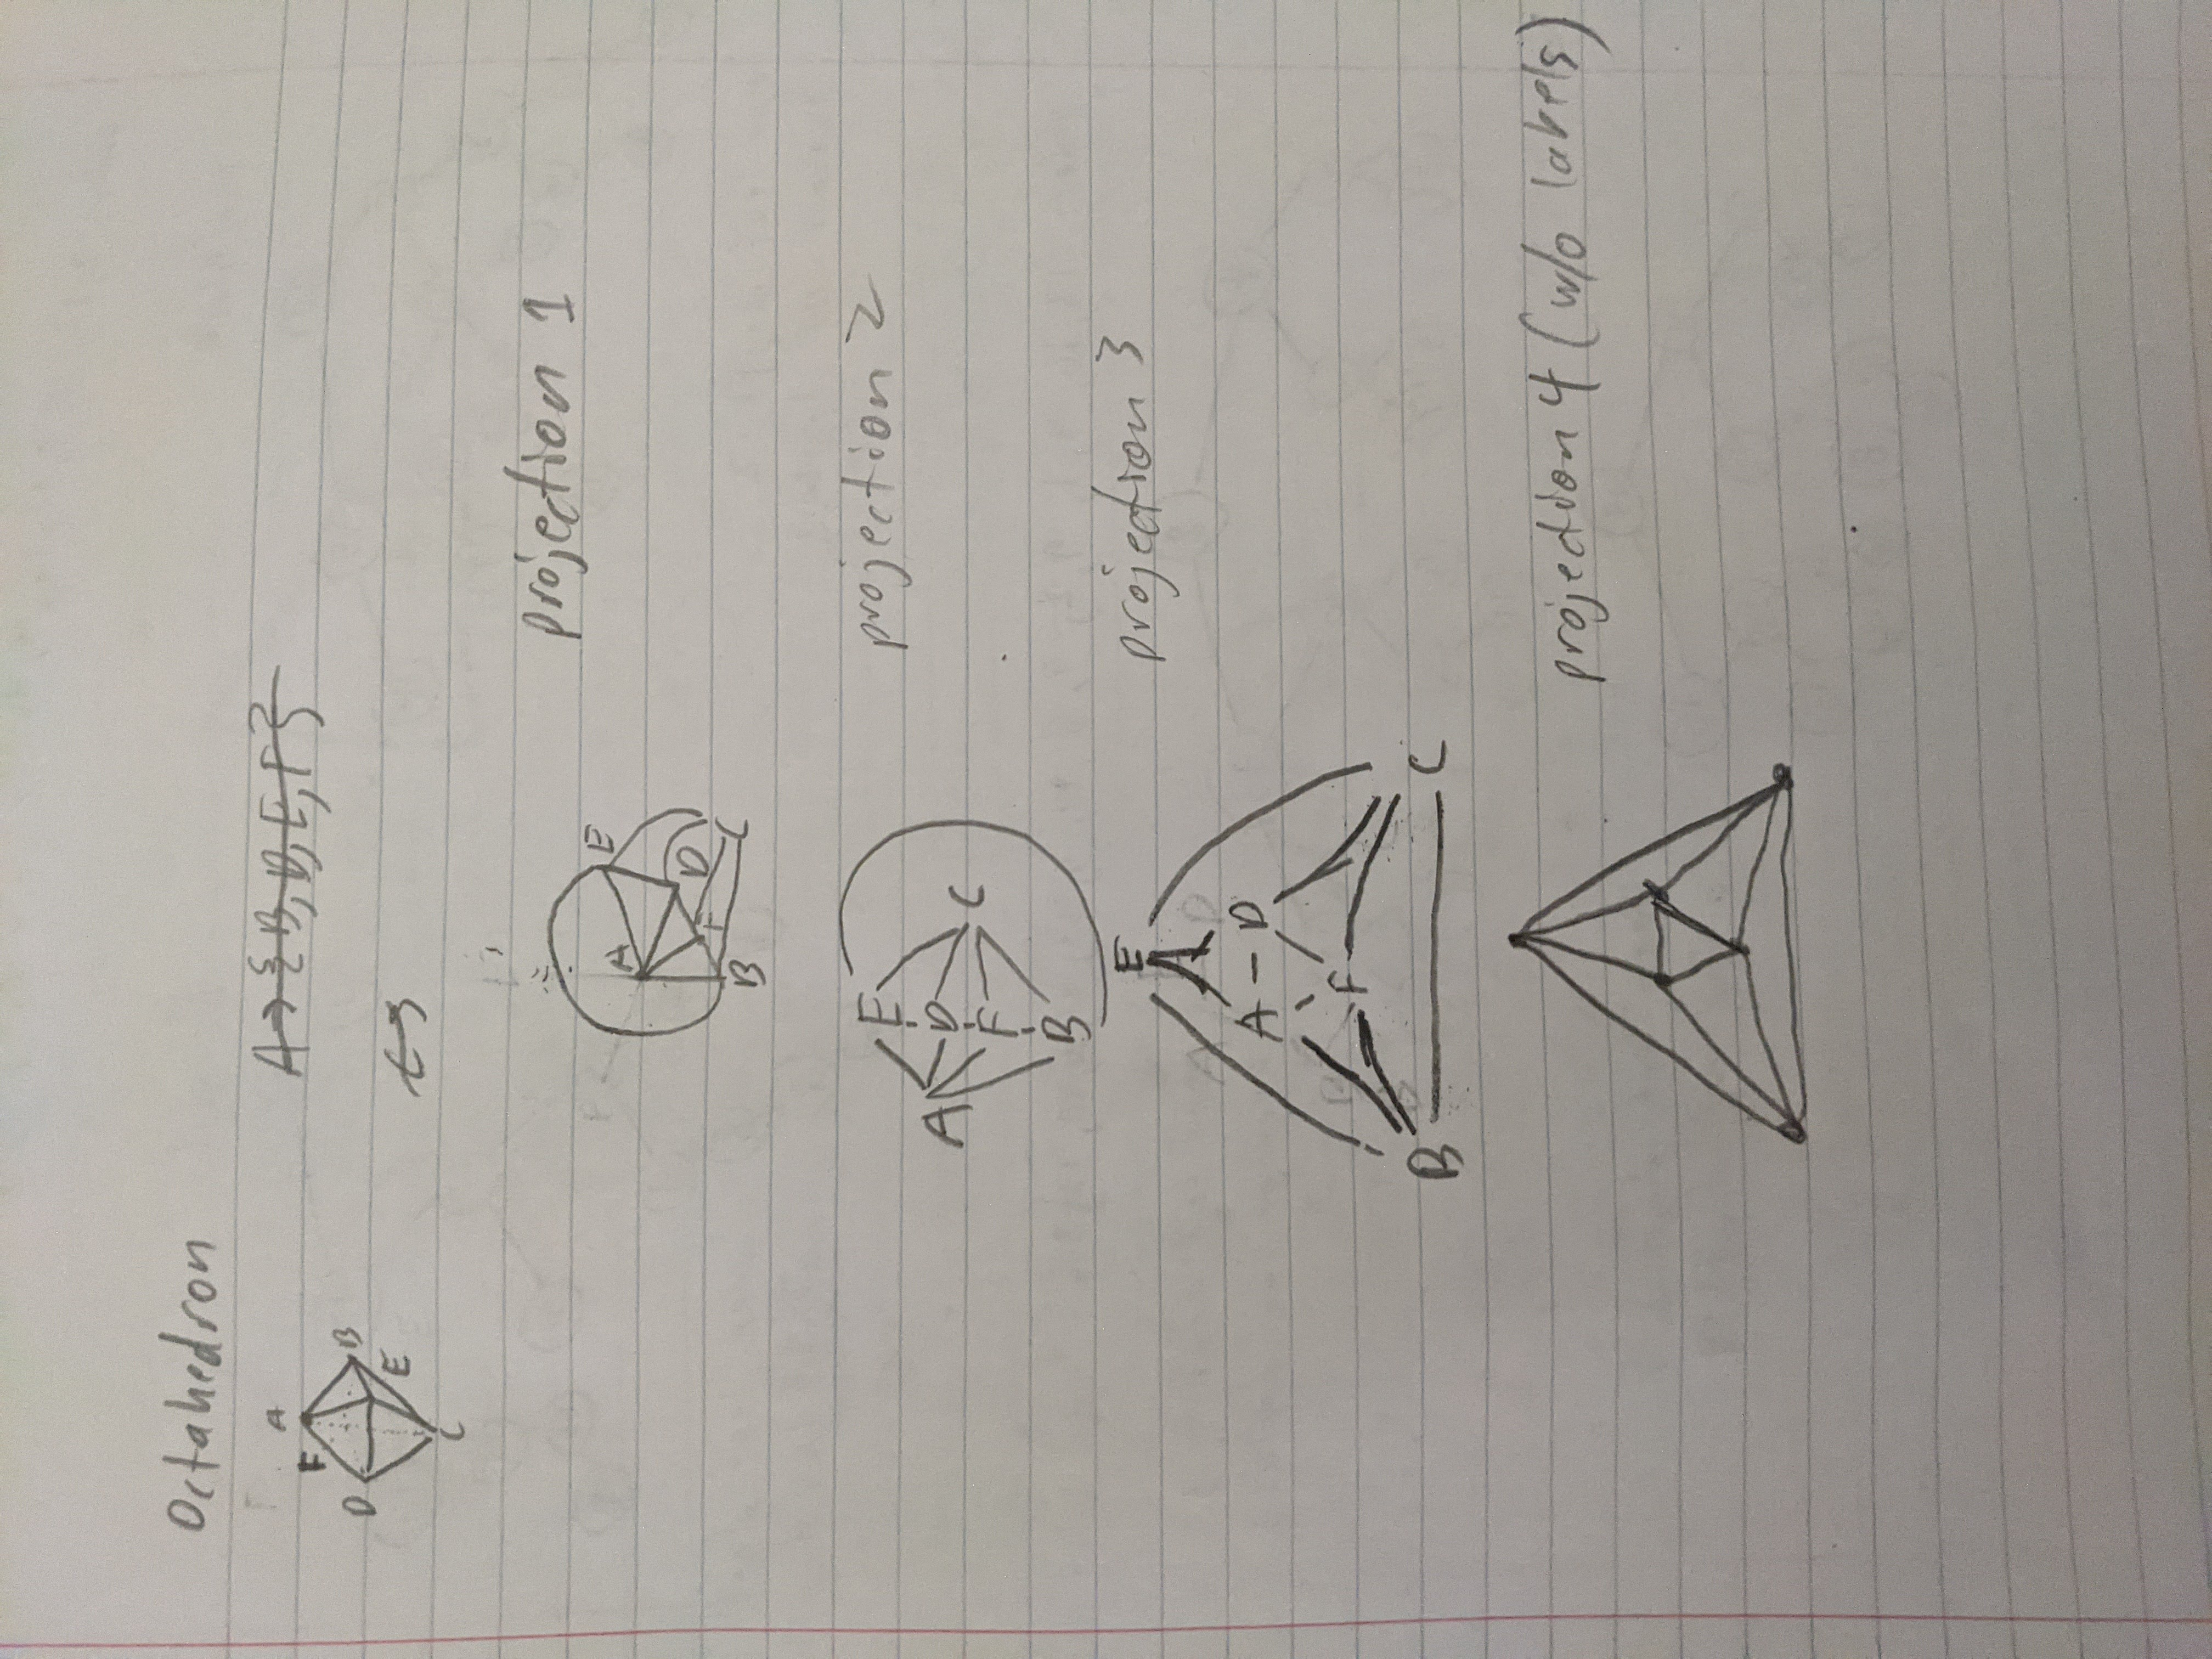
\includegraphics[width=\textwidth,angle=-90]{images/octahedron}
\label{graph}
\end{figure}



\end{enumerate}

% ============================================
% ============================================
\collab{n/a}
\nextprob{Fran Allen}
% ============================================
% ============================================

Write a short (1-2 paragraph) biography of Fran Allen.
\textbf{In your own words}, describe who they are and why they are important in
the history of computer science.

If you use external resources, please provide
proper citations. If you do not use external sources, please write ``I did not
use any sources to write this biography'' as the last sentence of the
biography.

\paragraph{Answer}

Frances Allen (1932-2020) was an American computer scientist born in New York. After graduating from the University of Michigan with a master's degree in mathematics, she worked for IBM.
While there, she spent time teaching IBM scientists FORTRAN and later contributed to the IBM's supercomputer compilers. She went on to found the Parallel TRANslation Group (PTRAN), where she focused
on efficient programming of computers that had multiple processors (Hosch). 

Her career was filled with awards. She was the first woman to be named an IBM fellow, and the president of the IBM Academy of Technology. She was the first woman to receive the A.M. Turing Award. She also was given the Augusta Ada Lovelace Award. She was also elected to many other positions such as to the IEEE and ACM (Hosch).

Hosch, W. L. (2020). Frances E. Allen. Retrieved March 19, 2021, from \url{https://www.britannica.com/biography/Frances-E-Allen}

% %% ... the bibliography
% \newpage
% \bibliographystyle{acm}
% \bibliography{biblio}

\end{document}

